%%% LaTeX Template: Article/Thesis/etc. with colored headings and special fonts
%%%
%%% Source: http://www.howtotex.com/
%%% Feel free to distribute this template, but please keep to referal to http://www.howtotex.com/ here.
%%% February 2011
%%%
%%% Modified October 2017 by SS

%%%  Preamble
\documentclass[11pt,letterpaper]{article}
\usepackage[margin=1.0in]{geometry}
\usepackage[T1]{fontenc}
\usepackage[bitstream-charter]{mathdesign}
\usepackage[latin1]{inputenc}					
\usepackage{amsmath}						
\usepackage{xcolor}
\usepackage{cite}
\usepackage{hyphenat}
\usepackage{graphicx}
\usepackage{float}
\usepackage{subfigure}
\usepackage{sectsty}
\usepackage[compact]{titlesec} 
\usepackage[tablegrid]{vhistory}
\allsectionsfont{\color{accentcolor}\scshape\selectfont}

%%% Definitions
\definecolor{accentcolor}{rgb}{0.0,0.0,0.5} 
\newcommand{\teamname}{Team Fisheye}
\newcommand{\productname}{FishMeasure}
\newcommand{\coursename}{CSE 4316: Senior Design I}
\newcommand{\semester}{Fall 2017}
\newcommand{\docname}{Project Charter}
\newcommand{\department}{Department of Computer Science \& Engineering}
\newcommand{\university}{The University of Texas at Arlington}
\newcommand{\authors}{Swangya Saurav \\ Brandon Timmons \\ Sujan Shrestha \\ Andrew Conroy}

%%% Headers and footers
\usepackage{fancyhdr}
	\pagestyle{fancy}						% Enabling the custom headers/footers
\usepackage{lastpage}	
	% Header (empty)
	\lhead{}
	\chead{}
	\rhead{}
	% Footer
	\lfoot{\footnotesize \teamname \ - \semester}
	\cfoot{}
	\rfoot{\footnotesize page \thepage\ of \pageref{LastPage}}	% "Page 1 of 2"
	\renewcommand{\headrulewidth}{0.0pt}
	\renewcommand{\footrulewidth}{0.4pt}

%%% Change the abstract environment
\usepackage[runin]{abstract}			% runin option for a run-in title
%\setlength\absleftindent{30pt}			% left margin
%\setlength\absrightindent{30pt}		% right margin
\abslabeldelim{\quad}	
\setlength{\abstitleskip}{-10pt}
\renewcommand{\abstractname}{}
\renewcommand{\abstracttextfont}{\color{accentcolor} \small \slshape}	% slanted text

%%% Start of the document
\begin{document}

%%% Cover sheet
{\centering \huge \color{accentcolor} \sc \textbf{\department \\ \university} \par}
\vspace{1 in}
{\centering \huge \color{accentcolor} \sc \textbf{\docname \\ \coursename \\ \semester} \par}
\vspace{0.5 in}
\begin{figure}[h!]
	\centering
   	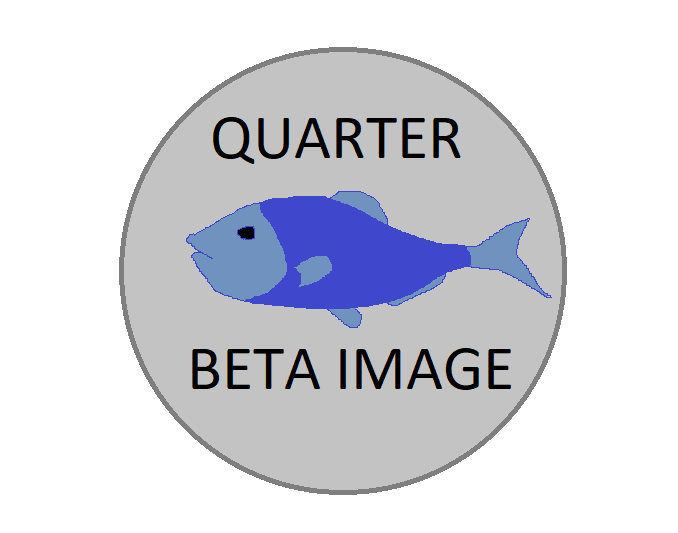
\includegraphics[width=0.60\textwidth]{images/test_logo}
\end{figure}
\vspace{0.5 in}
{\centering \huge \color{accentcolor} \sc \textbf{\teamname \\ \productname} \par}
\vspace{0.5 in}
{\centering \large \sc \textbf{\authors} \par}
\newpage


%\vspace{1 in}
%\centerline{January 13th, 2012}
%\newpage

%%% Revision History
\begin{versionhistory}
  	\vhEntry{0.0}{10.06.2017}{SwS,AC, BT, SuS}{document creation}

\end{versionhistory}
\newpage

%%% Table of contents
\tableofcontents
\newpage

%%% Agile project charter sections
\section{Vision}
Fishing is supposed to be fun and relaxing activity, but somehow the relaxing part is lost in trying to obey the laws regarding the minimum fish length. After catching a fish an arduous process of measuring the fish length beings, as it is illegal to keep a fish that is smaller than certain length. This saps out the relaxing part from the activity of fishing. Through this project we aim to make fishing a relaxing activity again. 
\section{Mission}
The aim is to create a mobile application that can be installed on an iPhone or Android device. Users will be able to snap the picture of the fish and would have to put a Quarter next to it at same depth from the device and the application will measure the length of the fish in terms of the length of quarter. Using that information it will be possible to calculate the approximate length of the fish.
\section{Success Criteria}
The app shall be available for at least one phone operating system, and should be available for the two major phone operating systems. The app shall be able to process a phone photograph of a fish on a wooden surface, with a quarter in the frame of the picture. The processed picture shall be able to identify the fish in the picture, and shall be able to identify the quarter in the picture. The app shall allow an option to post the image to a gallery that other viewers may use, and should be able to post the image to other social media. The app shall allow other app users to comment on the images posted to the gallery, for the purpose of identifying the species of the fish.
\newpage

%%% Remaining project charter sections
\section{Background}
Sport fishermen have complained that they have limited access to measuring equipment while on fishing excursions, and lack convenient systems to measure and identify their catch. Fishermen have expressed interest in a phone application that can use common objects (e.g. a coin) to measure the length of their catch, and a hotline of support from other fishermen to identify the catch, as many areas have laws on what is a lawful catch or not. This app seeks to use computer vision and social media functionality to fulfill these needs.
\section{Related Work}
Some related projects are FishFigure, Fish measurement, Hapyson fishing measurement and BAKUCHO measure. Most of these apps do not have image recognition feature. Hapyson fishing measurement app measures the length of fish based on the marker but we have to buy their marker. Our app will able to use common objects as a marker. The other feature that our app will be different is that it will have a feature to ask help from other fishermen to identify the catch.
\section{System Overview}
The system will be an android app that will help fishermen to measure the length of their catch. Fishermen can take a picture of the fish along side with a common object like a coin. The app will determine the length of the fish. The app will also have a feature to ask help from other fishermen to identify the catch. The app will use OpenCV for image recognition.
\section{Roles \& Responsibilities}
As the project evolves, team members may move between roles as the project evolves and developer experiences grow. The role of scrummaster will change each scrum, or every other scrum as decided by the team.
Andrew will prototype the user interface for the system, and the user storage for photographs uploaded into the system. He will also assist Timmons in the creation of the comment section for the gallery uploaded photos, and will work together to create the online gallery.
	Sujan will lead the android app development and aid Swangya in image recognition using OpenCV. He has experience in software development; creating systems in Android and Java. He will be in charge of building the wireframes for the software systems and come up with how the systems will interface with each other other. Along with managing the software systems, Sujan will also be a developer in creating these systems.
	Timmons will be the primary developer for the commenting feature for the app and help to create the online gallery. This will require establishing and utilizing a connection to the internet to upload and receive new photos and comments. He has experience in Android and Java to create and display images properly as well as scroll through a list of images or comments.

\section{Facilities \& Equipment}
Since this is a much more software based project, we will primarily only need our personal computers for programming and updating code. To test the project, we will use our smartphones to run the software and use the camera to take photos for size calculation and commenting. We will not be needing any special equipment that requires a lab, only a table to work at. There are plenty of locations on campus to work out and will be primarily meeting at the central library.
\section{Cost Proposal}
The camera required for the programming and processing power should be found in the standard smartphone so we will not require a new device to be purchased. The primary purpose of the app will be to take a photo of a fish next to a quarter to calculate the size of the fish. We will likely need a fish, real or fake, and a quarter. The project is cheap because it is designed not to require any new products or hardware for clients to use it so it is more available and convenient.
\section{Documentation \& Reporting}
In this section, you will describe all of the various artifacts that you will generate and maintain during the project lifecycle. Describe the purpose of each item below, how the content will be generated, where it will be stored, how often it will be updated, etc. 

\subsection{Project Charter}
The charter shall remain online for all team members to update, and will be audited by the site's History and Revisions section. The charter shall be updated as needed for the benefit of project clarity as the project approaches completion.

\subsection{Product Backlog}
A backlog shall be maintained using the Trello App, a plugin through the group's slack website. The team shall
list urgency of backlogged tasks in descending order.

\subsection{Sprint Planning}
Sprint planning sessions shall be held after every other scrum, decisions shall be made by a group vote, ties will be resolved either by random chance, or council with a third party.

\subsubsection{Sprint Goal}
Sprint goals shall be determined by team vote.

\subsubsection{Sprint Backlog}
The sprint backlog will be determined by the current scrum master, and will be descending order of urgency.

\subsubsection{Task Breakdown}
Tasks will first be assigned by volunteer, then by assessment of skills, or failing that, random chance.

\subsection{Sprint Burndown Charts}
The standing scrum master will construct the sprint burndown chart for the current sprint.

\subsection{Sprint Retrospective}
Sprint retrospectives will be held immediately before the next sprint.

\subsection{Individual Status Reports}
Status reports will be given each meeting, important information should be presented at the start of the meeting.

\subsection{Engineering Notebooks}
Every team member will maintain their own notebook, and will be signed by fellow team members.

\subsection{Closeout Materials}
No physical material will be shipped out, as it is a software application.

\subsubsection{System Prototype}
The prototype system will only have computer vision functionality, later prototypes may have UI and social media functionality.

\subsubsection{Project Poster}
The team shall design a poster to display the difference between out product and those mentioned in related work.

\subsubsection{Web Page}
We will make a simple webpage with instructions on how to use the app, the app may contain a link to the website, and the website may have a download link for the app.

\subsubsection{Demo Video}
A demo video may be made and imbedded into the website.

\subsubsection{Source Code}
The source code will be kept in google docs for the team to access, and the source code will be evaluated at the end of the project, and be made open source or kept private depending on factors made in development.

\subsubsection{Source Code Documentation}
The source code will be documented as modules are installed to the system.

\subsubsection{Hardware Schematics}
There are no hardware components required for this project, no schematics will be designed.

\subsubsection{CAD files}
There are no physical components requiring CAD files, no CAD files will be designed.

\subsubsection{Installation Scripts}
The scripts for installation will be made to work with an app store or by website download.

\subsubsection{User Manual}
Instructions for use may be included on the website, and will consist of a few paragraphs of instructions.
\newpage

%%% References
\bibliographystyle{plain}
\bibliographystyle{reference/IEEEtran_custom}
\bibliography{reference/refs}{}

\end{document}